\chapter{Xây dựng hệ thống server ảo}

\section {Giới thiệu kiến trúc hệ thống}

\subsection{Kiến trúc sử dụng cho nền tảng Github và Gitlab}
%\begin{figure}[htbp]
%	\centering
%	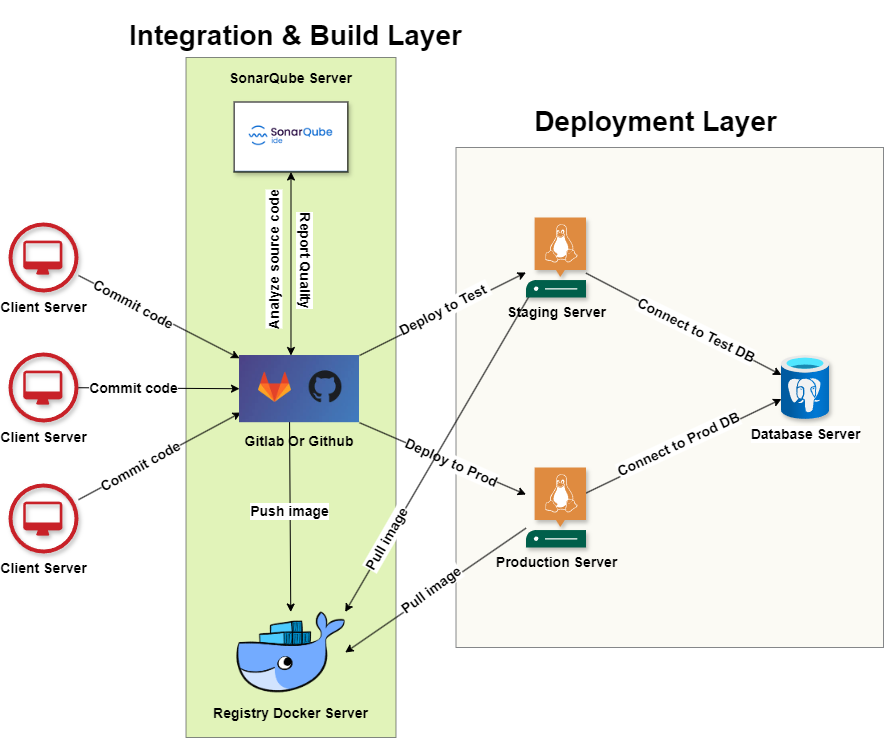
\includegraphics[width=1\linewidth]{Ảnh/gitlab-github-system-achitecture.png}
%	\caption{Kiến trúc hệ thống cho Gitlab và Github}
%	\label{fig:gitlab-github-system-achitecture}
%\end{figure}
%
%Hệ thống trên triển khai sử dụng hai nền tảng quản lý mã nguồn phổ biến là \textbf{GitHub} và \textbf{GitLab}, trong đó GitHub sử dụng \textbf{GitHub Cloud}, còn GitLab được cài đặt dưới dạng \textbf{GitLab Server} nội bộ trên hệ thống ảo. 
%
%
%Ở phía ngoài cùng bên trái của Hình~\ref{fig:gitlab-github-system-achitecture} là các máy khách (client).
%Các máy khách này do các lập trình viên (developer) sử dụng để phát triển phần mềm và thực hiện các thao tác như \textbf{pull/push} mã nguồn lên các nền tảng lưu trữ như GitHub hoặc GitLab.
%Việc kết nối giữa máy khách và máy chủ được thực hiện thông qua các \textbf{giao thức bảo mật SSH hoặc HTTPS}, giúp đảm bảo tính an toàn và xác thực khi truyền tải dữ liệu mã nguồn.
%
%
%Kiến trúc chính của hệ thống được chia thành hai lớp: \textbf{Integration \& Build Layer} và \textbf{Deployment Layer}, với các máy chủ được cấu hình và kết nối như Hình~\ref{fig:gitlab-github-system-achitecture}.
%
%\subsubsection*{Integration \& Build Layer}
%
%Lớp này là trung tâm của quá trình phát triển và kiểm thử phần mềm. 
%Nó bao gồm các máy chủ và dịch vụ chịu trách nhiệm lưu trữ mã nguồn, kiểm tra chất lượng, và đóng gói ứng dụng.
%\begin{itemize}
%	\item GitHub Cloud/ GitLab Server
%	
%	Hai máy chủ này đóng vai trò là \textbf{trung tâm quản lý mã nguồn}. Toàn bộ mã được lưu trữ và quản lý theo từng nhánh (\textit{branch}) hoặc phiên bản (\textit{commit}). 
%	
%	\begin{itemize}
%		\item Đối với \textbf{GitLab}, hệ thống được \textbf{cài đặt trên máy ảo nội bộ} (VMWare Workstation Pro), giúp nhóm phát triển kiểm soát hoàn toàn dữ liệu, tài nguyên và cấu hình CI/CD.
%		\item Đối với \textbf{GitHub}, nền tảng sử dụng \textbf{GitHub Cloud}, cho phép quản lý mã nguồn trực tuyến, không cần tự triển khai máy chủ và dễ dàng tích hợp với GitHub Actions.
%	\end{itemize}
%	
%	Nhiệm vụ của hai máy chủ Github Cloud và GitLab Server là lưu trữ máy nguồn 
%	
%	\item SonarQube Server
%	 
%	 \textbf{SonarQube Server} là máy chủ chuyên dùng để \textbf{phân tích chất lượng mã nguồn}. 
%	Khi mã được đẩy lên GitHub hoặc GitLab, hệ thống sẽ gửi yêu cầu tới SonarQube để thực hiện các bước kiểm tra như:
%	
%	\begin{itemize}
%		\item Phát hiện lỗi logic, bug, hoặc lỗ hổng bảo mật.
%		\item Đánh giá độ phức tạp và tính nhất quán trong cấu trúc mã.
%		\item Kiểm tra mức độ tuân thủ các quy tắc lập trình (code convention).
%	\end{itemize}
%	
%	SonarQube trả lại kết quả phân tích cho GitLab/GitHub dưới dạng báo cáo trực quan. 
%	Trong hệ thống ảo, máy chủ này được \textbf{tách biệt hoàn toàn} nhằm giảm tải và đảm bảo tính độc lập khi hoạt động.
%	
%	
%	
%	\item Registry Docker Server
%	
%	Máy chủ \textbf{Registry Docker} chịu trách nhiệm \textbf{lưu trữ hình ảnh (image) ứng dụng sau khi được build}. 
%	GitLab hoặc GitHub sẽ đóng gói ứng dụng thành Docker image và \textbf{push} lên máy chủ này. 
%	
%	Ưu điểm của việc tách riêng Registry là:
%	\begin{itemize}
%		\item Dễ quản lý và kiểm soát phiên bản ứng dụng.
%		\item Hỗ trợ triển khai nhanh đến các môi trường khác nhau.
%		\item Đảm bảo an toàn dữ liệu khi một máy chủ khác gặp sự cố.
%	\end{itemize}
%	
%	Trong hệ thống thực nghiệm, Registry được cài đặt nội bộ, tuy nhiên có thể thay thế bằng các dịch vụ cloud như \textit{Docker Hub} hoặc \textit{AWS ECR}.
%\end{itemize}
%
%\subsubsection{Deployment Layer}
%
%Lớp này bao gồm các máy chủ đảm nhiệm việc triển khai và vận hành ứng dụng ở các môi trường khác nhau. 
%Mỗi máy chủ được cài đặt độc lập nhằm tăng khả năng cô lập và đảm bảo an toàn hệ thống.
%
%\begin{itemize}
%	
%	\item Staging Server
%	
%	Đây là máy chủ \textbf{môi trường kiểm thử (staging environment)}. 
%	Tại đây, ứng dụng được triển khai để nhóm phát triển và kiểm thử viên đánh giá tính ổn định, chức năng và hiệu năng trước khi phát hành chính thức. 
%	
%	Máy chủ này \textbf{kết nối với cơ sở dữ liệu thử nghiệm (Test DB)} để đảm bảo việc kiểm thử không ảnh hưởng đến dữ liệu thật.
%	
%	
%	\item Production Server
%	
%	Máy chủ \textbf{production} là nơi \textbf{ứng dụng được vận hành thật}, phục vụ người dùng cuối. 
%	Sau khi phiên bản ở staging được xác nhận ổn định, image mới nhất sẽ được triển khai tại đây. 
%	
%	Máy chủ này \textbf{kết nối với cơ sở dữ liệu thật (Prod DB)} và thường được bảo mật, giám sát chặt chẽ hơn.
%	
%	\item Database Server
%	
%	Máy chủ cơ sở dữ liệu đảm nhiệm \textbf{lưu trữ dữ liệu cho cả hai môi trường}. 
%	Cấu trúc cơ sở dữ liệu được tách biệt thành hai phần:
%	\begin{itemize}
%		\item \textbf{Test DB:} phục vụ cho môi trường kiểm thử.
%		\item \textbf{Prod DB:} phục vụ cho môi trường thật.
%	\end{itemize}
%
%	
%\end{itemize}





\subsection{Kiến trúc sử dụng cho nền tảng Jenkins}

\section{Cài đặt hệ thống server ảo}